\documentclass[11pt]{article}

\usepackage{microtype}
\usepackage{amsmath}
\usepackage{xcolor}
\usepackage{graphicx}
\usepackage{enumitem}
\usepackage{latexsym}
\usepackage{xcolor}
\usepackage{float}
\usepackage{hyperref}
\hypersetup{
 colorlinks=true,
 citecolor=violet,
 linkcolor=red,
 urlcolor=blue}
\setlength{\parindent}{0cm}
\renewcommand\thesubsection{\alph{subsection})}

\title{\textbf{Assignment 6\\}Search Algorithms}
\author{Malik Al-hallak 90020\\
		Sebastian Utzig 100059\\
		Clemens Wegener 91268}
\date{}
\begin{document}
\maketitle

\section{Heuristics}
\subsection{}
Never, since $h(n)$ is dependent of the state $n$. 
\subsection{}
$g(n)$ can change when we reopen a node on CLOSED. Furthermore $g(n)$ can change while $n$ is on OPEN.
\subsection{}
$g(n)$ can change when we reopen a node on CLOSED. Furthermore $g(n)$ can change while $n$ is on OPEN.
\subsection{}
The cost $g(n)$ can change as long as the node $n$ is on the OPEN list. With a monotone $h$, a node that is put on CLOSED is reached with the cheapest path and hence will never be reopened.
\section{Admissibility}
No, since the $Z$ algorithm does not use \emph{delayed termination} it will return the first goal node, without considering possible cheaper solutions which are still on OPEN. So $Z$ will return \emph{a} solution but it may will not be the optimal solution. The example below show that $Z$ would return $\gamma$ instead of $\gamma^*$, because $\gamma$ is reached before $\gamma^*$. The used heuristic in this example is optimistic and hence admissible.

\begin{figure}[H]
	\centering
  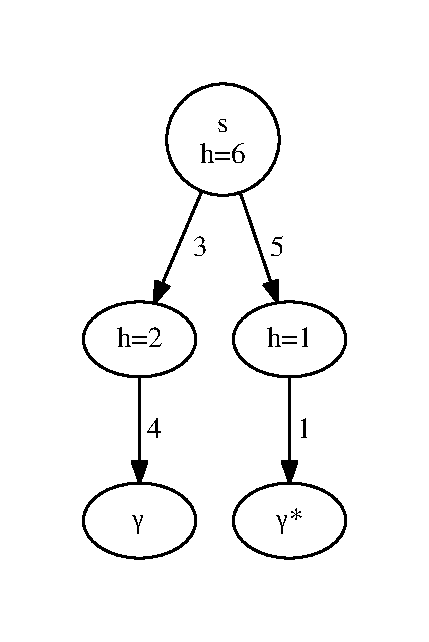
\includegraphics[width=0.4\textwidth]{./graph.pdf}
  \caption{Example $Z$ is not admissible}
	\label{fig2}
\end{figure}


\section{Monotonicity}
\subsection{}
Monotonicity defines a restriction on $h(n')$: When moving fron $n$ to $n'$ along the edge $(n,n')$ the $h$-value decreases at most by $c(n,n')$. 
\subsection{}
\paragraph{$h$ is admissible:}
There are states where the heuristic and true costs are equal. In this case each knight move decreases and never increases the distance to the goal state. Here the heuristic is optimistic because it does not overestimate the true costs. The second case describes all states which are adjacent to the goal state. Here the knight has to increase the distance again to reach the goal node. But the heuristic underestimates the true costs with maximal $\frac{2}{3}$ but the true costs are always greater than $1$.
\paragraph{$h$ is monotone:}
Each knight move increases the costs by $1$. The heuristic decreases each move at most by $1$ when moving towards the goal state in both dimensions. In other cases the heuristics decreases by less than $1$.  

\setcounter{section}{4}
\subsection{}
\begin{align*}
	h(n)=\left(1-\frac{16-d_{Man}}{16}\right)^2 \cdot \frac{d_{Man}}{3}
\end{align*}
\section{Relaxed Models}
Since $f_\omega = (1-\omega)\cdot g(n) + \omega\cdot h(n)$ with $\omega \rightarrow 1$ we perform a $BF^*$. Therefore, we propose the following conditions for the search:
\begin{itemize}
	\item $h$ is really near to the real costs (is very trustworthy)
	\item a maximum search depth is defined (for infinite graphs)
	\item a occurrence check is available to avoid cycle
\end{itemize}

\setcounter{section}{6}
\section{Implementing DWA$^*$ Search}
\subsection{}
Yes, we expect that DWA$^*$ expands the same number of nodes as A$^*$. Since the difference is the heuristic and hence the order the nodes are considered, both algorithms will work on the same nodes in different order. If the goal state is not reachable all nodes are processed from both algorithms until the OPEN list is empty and the algorithms fail.
\subsection{}
We would expect that DWA$^*$ performs the same amount of node expansions like A$^*$, because the $f$-value of both algorithms is identical.
\subsection{}
We would expect that DWA$^*$ performs less node expansions than A$^*$ because the heuristic $h(n)$ is weighted twice in the $f$-function and $h\approx h^*$.

\subsection{}
\begin{figure}[H]
	\centering
  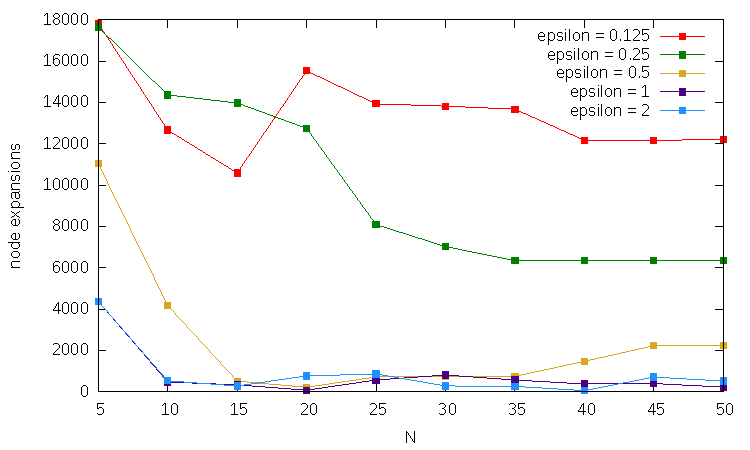
\includegraphics[width=\textwidth]{./result_eps.pdf}
  \caption{Number of node expansions for N $\in \;[5,10,...50]$ and $\epsilon \in \; [\frac{1}{8},\frac{1}{4},\frac{1}{2},1,2]$}
	\label{fig2}
\end{figure}

\subsection{}
DWA$^*$ terminates with an optimal solution of $31$ moves and $56$ expanded states with $N=40$ and $\epsilon=2$

\subsection{}
The same as in e)
\end{document}
